
\documentclass[journal]{IEEEtran}

\setlength{\fboxrule}{0pt}
\setlength{\fboxsep}{0pt}
\usepackage{color,soul}
\usepackage{tikz}
\usetikzlibrary{shapes.geometric, arrows, shapes.arrows, decorations.markings, calc}
\usepackage{pgfplots}

\hyphenation{op-tical net-works semi-conduc-tor}
\usepackage[english]{babel}
\usepackage{graphicx}
\usepackage{subcaption}
\usepackage{hyperref}
\usepackage{cite}
\usepackage{multirow}

\tikzstyle directed=[postaction={decorate,decoration={markings, 
		mark=at position 1 with {\arrow[arrowstyle]{stealth}}}}]

\tikzstyle arrowstyle=[scale=1]

%for flowcharts
\tikzstyle{testing} = [
thick,
->,
>=stealth
]
\tikzstyle{training} = [
thick, 
decoration={
	markings,
	mark=at position 1 with {
		\arrow[semithick]{open triangle 60}
	}
},
double distance=1.4pt, 
shorten >= 5.5pt,
preaction = {decorate},
postaction = {
	draw,
	line width=1.4pt,
	white,
	shorten >= 4.5pt
}
]

\tikzstyle{data} = [
cylinder, 
shape border rotate=90, 
draw,
minimum width=1.5cm, 
minimum height=1.2cm,
text centered, 
draw=black, 
line width=0.3mm,
shape aspect=.1
]

\tikzstyle{operation} = [
rectangle, 
rounded corners,
minimum width=2cm, 
minimum height=1.2cm,
text centered, 
draw=black, 
line width=0.6mm,
]

\tikzstyle{sample} = [
rectangle, 
minimum width=1.2cm, 
minimum height=1.2cm,
text centered, 
draw=black,
line width=0.3mm,
]

\tikzstyle{metric} = [
diamond, 
minimum width=1.2cm, 
minimum height=1.2cm,
text centered, 
draw=black,
line width=0.3mm,
]

\tikzstyle{filter} = [
trapezium, 
trapezium left angle=70, 
trapezium right angle=110, 
minimum width=1.5cm, 
minimum height=1cm, 
text centered, 
draw=black, 
line width=0.5mm
]

\begin{document}

\title{Generative adversarial neural networks model of photonic crystal fiber based Surface Plasmon Resonance Sensor}
\author{
	Aimen Zelaci, Ahmet Yasli, Cem Kalyoncu, and Huseyin Ademgil, \IEEEmembership{Senior Member, IEEE}
	\thanks{A. Z. Author is with 
		the European University of Lefke, Faculty of Engineering, Electrical and Electronics Engineering Department, Lefke, TR-10, Turkey (e-mail: aimen.zelaci@gmail.com).
	}
	\thanks{A. Y. Author is with 
		the European University of Lefke, Faculty of Engineering, Electrical and Electronics Engineering Department, Lefke, TR-10, Turkey (e-mail: ayasli@eul.edu.tr).
	}
	\thanks{C. K. Author is with 
		the European University of Lefke, Faculty of Engineering, Computer Engineering Department, Lefke, TR-10, Turkey (e-mail: ckalyoncu@eul.edu.tr).
	}
	\thanks{H. A. Author is with 
		the European University of Lefke, Faculty of Engineering, Computer Engineering Department, Lefke, TR-10, Turkey (e-mail: hademgil@eul.edu.tr).
	}
}



% The paper headers
\markboth{ Journal of Lightwave Technology,~Vol.~14, No.~8, August~2015}%
{Shell \MakeLowercase{\textit{et al.}}: Bare Demo of IEEEtran.cls for IEEE Journals}




% make the title area
\maketitle

\begin{abstract}
	Photonic crystal fibers (PCF) for specific applications are designed and optimized by both industry experts and researchers. However, the potential number of design combinations and flexible propagation features are offering a wide range of application areas, resulting in an exponential increase in the search space. This issue combined with the speed of the commonly used Full Vectorial Finite Element Method (FV-FEM) simulators causes the task to take a significant amount of time. As stated in the previous works, artificial neural networks (ANN) can be employed to predict the result of numerical simulations much faster. However, there are two issues with the methods proposed previously: the required number of samples for training and the generality of these methods. In this paper, we propose the use of generative adversarial networks (GAN) to augment the real dataset to train an ANN model. The experimental analysis suggested that the proposed combination not only accurately predicts the confinement loss even with limited amounts of data but also GAN can be used to improve existing methods in the literature. Moreover, the proposed system can also predict the confinement loss over a range of analytes and wavelengths in a completely new geometric configuration and generic enough not to require any additional tuning when used in a new dataset. This property is demonstrated by experimenting on an existing PCF dataset, which the proposed system surpassed the accuracy of the method proposed for it.
\end{abstract}

\begin{IEEEkeywords}
	Artificial neural network (ANN), fiber optic sensor, generative adversarial networks (GAN), machine learning, photonic crystal fiber (PCF), surface plasmon resonance (SPR).
\end{IEEEkeywords}






% For peer review papers, you can put extra information on the cover
% page as needed:
% \ifCLASSOPTIONpeerreview
% \begin{center} \bfseries EDICS Category: 3-BBND \end{center}
% \fi
%
% For peerreview papers, this IEEEtran command inserts a page break and
% creates the second title. It will be ignored for other modes.
\IEEEpeerreviewmaketitle



\section{Introduction}
Due to their unique propagation features, Photonic Crystal Fibers (PCFs) have been integrated into a number of optical based devices and applications. Design flexibilities and precise light guidance abilities has made them more promising in comparison to conventional step index fibers in various optical applications including sensing \cite{wang2011selectively}. 

In the last decade, PCF based structures are extensively employed as sensing devices. Possibility of filling the cladding holes with gas and liquid analytes makes them favorable in both chemical and biological sensing applications  \cite{wang2011selectively,rifat2016highly,caucheteur2015review,dash2014spr}. Moreover, due to adaptable light guidance with possibilities of controlling the confinement loss and the chromatic dispersion at any operating wavelength are distinguishing features of PCF based structures in the literature. These charming propagation features can be achieved by employing, circular, cylindrical and even square and rectangular shaped \cite{wang2015simulation} air holes in the cladding and in the core region of the structures. Furthermore, the cladding pattern arrangements such as hexagonal, octagonal, decagonal, square and circular \cite{wang2011selectively,bouk2004dispersion,ademgil2014highly,razzak2007chromatic} can be engaged to achieve the desired features for preferred applications. The hole-to hole spacing (pitch) and the air hole sizes are critical parameters of tuning the aforementioned propagation characteristics. On the other hand, surface plasmon resonance (SPR) is a unique technique that occurs with light and free electrons interaction at metallic boundaries. This interaction results with excitement of surface plasmon polarition (SPP). Relative permittivity variations of the analytes will change the characteristics of the SPP wave, where sensing is triggered. Kretschamann Raether prism geometry is the fundamental construction principle of SPR based sensors  \cite{kretschmann1968radiative}. This geometry practices Snell's Total Internal Reflection rule, where still a very small amount of light refracts from the metallic layer into the evanescent field. The refracted photons are coupling with electron charge oscillations (plasmon) at the surface of the metallic layer, which are known as surface plasmon waves (SPW). The maximum energy transfer from core mode to SPWs occurs with the effective index equalization of these corresponding modes. This phenomenon is known as resonance phase matching, where losses are reaching the maximum levels. The possible changes in the analyte index will directly affect the resonance matching wavelengths. These possible variations are the main parameters for sensitivity calculations. The deep research on SPR based sensors have shown that Kretschmann Raether's prism geometry fails to satisfy the remote sensing and miniaturization requirements of critical detecting applications. One of the most common solutions of overcoming these limitations is replacing the prism with the core of an optical fiber. Considering the recent technological developments, PCF are offering a tremendous amount of design flexibility with the possibilities of complete control of light guidance. Hence, SPR technique can be integrated to this unique microstructured fibers for developing comprehensive multi-purpose sensor \cite{rifat2016highly,yasli2019effect}. Following the exclusive study by Hassani and Skorobogatiy \cite{hassani2006design}, a number of structures have reported the merits of PCF based SPR sensors. In the past, structures that contains features such as multi-channel single analyte and multi-channel multi analyte have been investigated \cite{rifat2016highly,yasli2019effect,zhang2011wagon,yasli2019multi,azzam2016multichannel}. Also, the effects of various metallic layers such as Au, Ag \cite{yasli2019multi}, Ag- Graphene \cite{rifat2016highly}, Ta2TO5 \cite{otupiri2015multi}, ITO \cite{dash2014spr}, TiO2 \cite{rifat2016highly} with various design parameters have also been investigated in detailed. Several design parameters such as plasmonic material, thickness of the layers, air hole size and positions are decisive on resonance matching wavelength of the SPR based structures. Optimizing and refinement of these parameters is an extremely time consuming process with considerable computational time \cite{fornarelli2009neural,abdelaziz2012photonic,paper0}. In the past, genetic algorithms \cite{abdelaziz2012photonic,borel2004topology} method was used to optimize the structural design parameters to achieve better propagation features of photonic devices \cite{rifat2016highly,caucheteur2015review}. Nowadays, in order to optimize such structures, artificial neural networks (ANN) and other machine learning (ML) algorithms are being applied \cite{fornarelli2009neural,paper0,hameed2008accurate}. Although ANNs and ML have been applied to PCFs \cite{fornarelli2009neural,paper0} and SPR structures \cite{fu2018optimization,mcatee2019artificial} independently, to the best of our knowledge, there seems to have been no published papers that investigated the PCF based SPR structures with this well tested methods.


Machine Learning (ML) techniques are becoming a common tool in many fields and surpassing human performance in many tasks, such as automatic speech recognition, image recognition, natural language processing, drug discovery and toxicology. Additionally, ANN can approximate any function proven by the Universality theorem  \cite{HORNIK1991251}. This fact propelled researchers to widen the applications of ANN even further, including the study of nano-photonic structures   \cite{kiarashinejad2020knowledge}, optimization of photonic crystal nano-cavities \cite{asano2018optimization}, and more recently, computing optical properties of a PCFs  \cite{paper0} and SPR structures \cite{fu2018optimization,mcatee2019artificial}.

One of the most difficult challenges that deep learning models are facing is that they benefit from large amounts of data to train, which is often costly and/or difficult to acquire. An alternative solution is to artificially expand the original training dataset by the means of generative networks. In this regard, Generative Adversarial Networks (GAN) introduced by Goodfellow et al  \cite{goodfellow2014generative}, has proven to be successful in data generation  \cite{schlegl2017unsupervised, zheng2017unlabeled, frid2018synthetic, tanaka2019data, perez2017effectiveness}.

In this work, we focused on estimating the confinement loss behavior of multichannel PCF based SPR sensors by employing the ANNs. Specifically, we have constructed our system on a PCF based SPR model. However, in the experiments section we have demonstrated that the designed system is generic enough to be applied to multiple similar PCF based designs. The most important contribution of this research is the use of the GAN phase, where the available data is expanded to be used in the training phase.

To our knowledge, Ref.~\cite{hameed2008accurate} was the first work proposed ANN technique on PCF structures. The results demonstrated the accuracy of the network on a specific PCF structure. On the other hand, ANN method was employed for predicting the chromatic dispersion of conventional hexagonal lattice PCF structure \cite{rodriguez2010efficient}. In Ref. \cite{mescia2011refinement},authors employed a neural network for the refinement and design of Erbium doped PCF. Presented results have shown that conventional methods consume large amounts of time compared to the runtime of the neural network. Perhaps the most rigorous experiments about neural network use in PCF design is presented in  \cite{paper0}.In this work, a feed-forward multi-layer perceptron neural network is used to calculate multiple propagation features of a PCF design. It can be seen that this proposed network can achieve both acceptable accuracy and superior speed compared to the existing numerical methods. On the other hand, genetic algorithms and ANN methods have also been tested on SPR sensor structures \cite{fu2018optimization,mcatee2019artificial}. These methods also deliver robust performances.

The accuracy of existing image classifiers of the neural networks can be improved by using GAN  \cite{perez2017effectiveness}. Frid-Adar, et. al. \cite{frid2018synthetic} have applied the same method to improve the accuracy of liver lesion classification. It is found that balancing the training data with GAN has a higher improvement in accuracy compared to classical data generation strategies. The same technique was applied to augment and anonymize the training data of the brain MRI  \cite{shin2018medical}.


This paper is organized as follows.The details of GAN procedure to generate additional training samples for ANN as well as the proposed neural network architecture is presented in Section \ref{sec:prop}. The design parameters and details of PCF based SPR structure is described in section \ref{sec:pcf}. Detailed analysis of the numerical results is discussed in section \ref{sec:exp}. Finally, concluding remarks are presented in Section \ref{sec:conc}.

\section{Network Architecture}
\label{sec:prop}

In this section, details of the proposed method are discussed. Training of the system contains two phases: a GAN phase and regression training phase. At the beginning of the training, a GAN is trained to generate additional data by using training samples. These generated samples are filtered to ensure they are within the numeric range of application. Original training samples and generated samples are joined to train a fully-connected feedforward multi-layer perceptron (MLP) neural network. This satisfies the regression need for estimating the confinement loss. At the end of the training, the ANN will be used to decide the confinement loss of a previously unseen set of input parameters. The illustration of the proposed architecture is presented in Figure \ref{fig:overall}. The details of the proposed GAN and ANN architecture is discussed in the following sub-sections.

\begin{figure}
	\centering
	\begin{tikzpicture}[node distance=2cm]
	\node (collected) [data] {Collected samples};
	\node (GAN) [operation,below of=collected,xshift=-2cm] {GAN};
	\node (filter) [filter, below of=GAN, text width=2.4cm] {\baselineskip=10pt Filter out-of-range samples\par};
	\node (generated) [data, below of=filter] {Generated samples};
	\node (ann) [operation,below of=generated,xshift=2cm] {ANN};
	\node (testsample) [sample, right of=generated,xshift=2cm,yshift=-1cm, text width=1.2cm] {\baselineskip=10pt Test\par};
	\node (output) [sample, below of=testsample,yshift=-0cm, text width=1.2cm] {\baselineskip=10pt Output\par};
	
	\node (legendtrain) [right of=GAN,xshift=2cm] {};
	\node (legendtrainend) [below of=legendtrain,yshift=1cm] {Training};
	\node (legendtest) [below of=legendtrainend,yshift=1cm] {};
	\node (legendtestend) [below of=legendtest,yshift=1cm] {Testing};
	
	
	\draw [training] (collected) -- (GAN);
	\draw [training] (GAN) -- (filter);
	\draw [training] (filter) -- (generated);
	\draw [training] (generated) -- (ann);
	\draw [training] (collected) -- (ann);
	\draw [testing] (testsample.west) to [bend right=45] ($(ann.north east)-(0.5,0)$);
	\draw [testing] ($(ann.south east)-(0.5,0)$) to [bend right=45] (output.west);
	
	\draw [training] (legendtrain) -- (legendtrainend);
	\draw [testing] (legendtest) -- (legendtestend);
	
	\end{tikzpicture}
	\caption{System architecture}
	\label{fig:overall}
\end{figure}


\subsection{Generative adversarial network design}
\label{ssec:gan}
In our study, GAN is employed to augment the number of samples that are used in training  \cite{goodfellow2014generative}. A GAN is composed of two neural networks: generator and discriminator. The aim of the generator is to transform fully randomized data into form that follows the distribution of the original dataset. The discriminator assesses the performance of the generator and provides feedback for training. Instead of directly training the generator, it is trained through this feedback. This paradigm avoids overfitting the data.

The GAN can be trained by diverse metrics \cite{goodfellow2014generative, mao2017least, lucic2018gans}]. In this work Wasserstein distance metric (WGAN) is employed \cite{arjovsky2017wasserstein}. In this system, discriminator is named as critic and it measures the distance between the generated and the real data. The distinguishing feature of the WGAN compared to other methods is the ability to determine a stopping criteria. In a regular GAN system, training is stopped when the generated data is deemed viable by an observer. GAN is frequently used in image, video or audio generation, where human is used effectively in the loop. In our case, it is not viable for a human to judge the generated data, therefore, automating this procedure to remove the human in-the-loop can lead to over or under-fitting, which may degrade the performance. On the other hand, WGAN uses an adaptive stopping criteria that can easily overcome the aforementioned disadvantages. Additionally, Gradient penalty is incorporated to improve the WGAN as described in \cite{gulrajani2017improved}. This proposed enhanced WGAN system converges in a stable manner without requiring further fine tuning the hyper-parameters of the system. % The flowchart of this proposed system is illustrated in Figure \ref{fig:gan}.

In our work, both the critic and the generator are fully connected feed forward MLP models. The detailed parameters of the networks are given in Table \ref{tbl:anndetails}. The output of the system would be input and output pairs that are used to train ANN part of the system. In our proposed model, we have 7 input parameters and a single output parameter, making a total of 8 that will be used in the GAN phase. In Section  \ref{sec:exp}, various PCF structures are tested with different inputs, resulting in a different number of system parameters. The generator is supplied with the same number of parameters. These parameters are generated using Gaussian noise and this input is called latent variable.

Previous works \cite{ravuri2019seeing, shmelkov2018good}, demonstrated that it is possible for random data augmentation to weaken the performance of the model. Hence, it is important to sample the generated data in a way to prevent performance degradation  \cite{bhattarai2019sampling}. In our proposed system, we have included a filtering step for the generated data. This step uses a simple condition to discard the values that fall out of the desired range of both the independent variables  ($n_{analyte}, \lambda, \Lambda, d1, d2, d3, n_c$), and the confinement loss. Once the training phase is completed, the generator and the filter is used to augment the number of training samples that are available for ANN to train on.
%
%\begin{figure}
%	\centering
%	\begin{tikzpicture}[node distance=2cm]
%	\node(latent) 	[filter,text width=1.4cm] 		{\baselineskip=10pt Noise generator\par};
%	\node(generator)[operation,below of=latent] 	{Generator};
%	\node(generated)[data, below of=generator,
%	text width=1.4cm]				{\baselineskip=10pt Generated samples\par};
%	\node(collected)[data, right of=generated,
%	xshift=1cm,text width=1.4cm]	{\baselineskip=10pt Collected samples\par};
%	\node(critic)	[operation,below of=generated,
%	xshift=1.5cm]					{Critic};
%	\node(metric)   [metric,below of=critic,
%	text width=1.4cm, yshift=-.2cm]{\baselineskip=10pt{}Wasserstein distance\par};
%	
%	\draw [training] (latent) -- (generator) node [pos=.5, left, xshift=-0.1cm] (z) {Latent variable};
%	\draw [training] (generator) -- (generated);
%	\draw [training] (generated) -| (critic);
%	\draw [training] (collected) -| (critic);
%	\draw [training] (critic) -- (metric);
%	\draw [testing]  (metric.east) - ++(1,0) |-  (critic.east);
%	\draw [testing]  (metric.west) - ++(-2.2,0) |-  (generator.west);
%	\end{tikzpicture}
%	\caption{WGAN training}
%	\label{fig:gan}
%\end{figure}

\begin{table*}
	\centering
	\caption{Details of ANN models}
	\begin{tabular}{l|l|l|l}
		\textbf{Parameter} & \textbf{Generator} & \textbf{Critic} & \textbf{Regressor} \\\hline
		Hidden layers & 5 & 5 & 5 \\
		Neurons in hidden layers & $ 128 $ & $2^{layer\_index} \times 32$ & 50 \\
		Batch size & 32 & 32 & 48 \\
		Activation function & ReLU & Leaky ReLU & ReLU \\
		Optimizer & Adam \cite{kingma2014adam} & Adam & Adam \\
		Input normalization & None & None & None \\
		Layer normalization & None & Batch \cite{ioffe2015batch} & Batch \\
		Loss function & $-Critic\left[gen\right]$ & $Critic\left[gen\right] - Critic\left[col\right] + Penalty_{grad}$ & MSE \\\hline
		\multicolumn{4}{l}{gen: generated, col: collected, grad: gradient}
	\end{tabular}
	\label{tbl:anndetails}
\end{table*}


\subsection{Artificial neural network design}
\label{ssec:ann}

The ANN model employed in this work is a fully connected feed-forward MLP network consisting of an input layer, an output layer, and 5 hidden layers. The ANN is designed and trained to estimate the confinement loss in a regression configuration. We have applied  $log_{10}$ to confinement loss calculation in order to keep its numeric stability across a wide range \cite{paper0}. Each hidden layer contains 50 neurons and uses Rectified Linear Unit (ReLU) activation function. Table  \ref{tbl:anndetails} summarizes the details of this model. \hl{The number of hidden layers and neurons are empirically determined to be able to estimate the loss curve while keeping the complexity of the network to minimum.}

In our model, we have used mini-batch training with 48 samples as the batch size. In contrast to full-batch training, mini-batch training allows more frequent gradient calculations, improving the stability and reliability of the training \cite{masters2018revisiting, keskar2016large}. The weakness of using mini-batches is added computational complexity during training. However, it has no adverse effect on the testing phase.

We have adopted Adam \cite{kingma2014adam}as the optimizer and mean squared error (MSE) as the loss/cost function. In addition, Batch Normalization algorithm \cite{ioffe2015batch} is employed to accelerate the training, reduce the effects of initial randomized state and mitigate the problem of internal covariate shift. Also, the ANN is trained using the training samples from the original dataset and the augmented samples generated by the GAN phase.

\section{Photonic crystal fiber design}
\label{sec:pcf}

In order to build the desired dataset, the numerical analysis of the proposed sensor structure is carried out with the commercial software package Comsol Multiphysics  \cite{comsol_help}. The Full Vectorial Finite Element Method (FV-FEM) with the perfectly matched layers (PMLs) \cite{koshiba2002full,saitoh2001full} are employed.

The cross section of the proposed structure is illustrated in Figure 3. As can be seen from this figure, the sensor consists of an analyte channel (sensing medium), plasmonic layer (Au)and various sized cladding air holes. The cladding region is formed by nineteen various sized air holes, sited on silica background with hexagonal lattice arrangement. The air hole diameters are set to;  $d_1$= $0.45 \mu m$, $d_2$= $0.75 \mu m$, $d_3$= $0.35 \mu m$, and  $d_c$= $0.15$. The distance between air holes ($\Lambda$) are fixed to $2 \mu m$. Initially, trapping the light (fundamental mode) into the core region is vital for mode quality. On the other hand, some amount of light needs to be leaked towards the plasmonic layer, where the sensitivity measurement occurs. This is the key phenomenon for resonance phase matching occurrence. In this respect, the various sized cladding holes are employed for controlling the light guidance, where each set of air holes are affecting different propagation characteristics of the sensor. The Gold (Au) material is used as a plasmonic layer and set to be $40 \mu m$. The Johnson and Christy Data \cite{johnson1972optical} are used for the permittivity values. The Sellmeier Equation (Eq.(\ref{eqn1})) is used for calculating the refractive index of Silica material \cite{bjarklev2003PCF}.

\begin{figure}[]
	\centering
	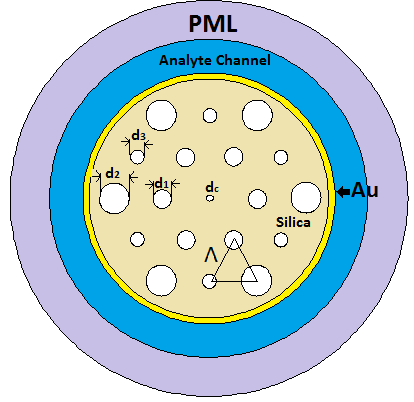
\includegraphics[width=.7\linewidth]{figures/Figx}
	\caption{The cross-section of proposed  PCF based SPR sensor.}
	\label{Figx}
\end{figure}




\begin{equation}
n^2(\lambda)=1+\frac{ B_1 (\lambda)^2} {(\lambda)^2-C_1} + \frac{ B_2 (\lambda)^2} {(\lambda)^2-C_2} + \frac{ B_3 (\lambda)^2} {(\lambda)^2-C_3}
\label{eqn1}
\end{equation}
%% 

where $\lambda$ is the operating wavelength, $n$ is the Refractive Index (RI), $B_{1,2,3}$ and  $C_{1,2,3}$ are the  Sellmeier constants~\cite{bjarklev2003PCF}.

As mentioned in the introductory part, during the resonance phase matching condition, the confinement losses are reaching the highest rate. Therefore, precise calculation of the confinement losses are critical. The Equation \ref{eqn2} is used in this study for that purpose \cite{yasli2019effect}.



%%
\begin{equation}
\frac{40\pi}{ln(10) \lambda} Im(n_{eff}) \times 10^{4} [dB/cm]
\label{eqn2}
\end{equation}
%%

where the imaginary part of the effective RI shown with Im($n_{eff}$).

A labelled dataset of 432 samples was provided by FVFEM numerical analysis. Our dataset contains a number of independent variables, such as the operating wavelength  $\lambda$, analyte index $n_{analyte}$, hole to hole distance $\Lambda$, the air holes sizes ($d_1$, $d_2$ and $d_3$), and the real part of the refractive index ($n_c$). The labels are specified as the confinement loss of the sensor structure. The set consists of nine different configurations of the geometric properties ($\Lambda$, $d_1$, $d_2$, $d_3$), for each configuration the confinement loss was calculated for three different analytes (Water (n=1.33), Ethanol (n=1.35) and several commercial hydrocarbon mixtures (n=1.36)).

The optimizing and refinement of these above parameters are extremely time-consuming and requires considerable computational time. In order to optimize the structural design parameters and achieve the desired propagation features, we have fixed the geometry of the sensor structure (hexagonal arrangement with circular air holes) and vary the operating wavelength $\lambda$, index of refraction $n_{analyte}$, hole to hole spacing $\Lambda$, and the size of the cladding holes ($d_1$, $d_2$ and $d_3$).


\section{Experiments}
\label{sec:exp}

\subsection{Experimental setup}

\def\dszero{PCF}
In order to prove the effectiveness of the proposed setup, we have performed multiple experiments over two datasets. We have built the first dataset that is used in the experiments. Details of this dataset is explained in Section \ref{sec:pcf} and it is referred to as SPR dataset. We have performed 9-fold testing on this dataset, due to having nine configurations. Each fold tests a single configuration using the other configurations as training data. Slicing the data allows us to guide the network to predict the loss on a configuration that has not been used in training. Please note that we have applied $log_{10}$ to confinement loss for scaling.

Also, mean square error (MSE) is used for the comparisons. All algorithms are implemented using TensorFlow with Keras library in Python and experiments are performed on device with Intel i7-5600 CPU and 8GB of RAM. TensorFlow library is set to use only CPU for the experiments.

Additionally, we have used the dataset that has been used in \cite{paper0}. This dataset contains 1117 samples. \hl{There are 5 inputs}: refractive index of the core ($n_c$), wavelength ($\lambda$), hole diameter ($d$), pitch ($\Lambda$), and number of rings ($N_r$);  and outputs are effective index ($n_{eff}$), effective mode area ($A_{eff}$), dispersion ($D$), and the confinement loss ($\alpha_c$). We have only used confinement loss as the output. This dataset is referred to as PCF. As a final note, the range and domain of these datasets are different; therefore, all numeric comparisons should be drawn within the same dataset.

In the following subsections, we have performed experiments to show the performance of the base ANN system by its own comparing with the state-of-the-art method in the literature \cite{paper0}, improvement gained by employing GAN phase, and finally the computational advantages of using ANN over the simulator. 5000 training epochs are used for  \cite{paper0} as suggested in the original paper. All numeric comparison results are averaged over multiple executions: 9-fold testing for SPR dataset and 10-fold testing for \dszero. Non-averaged data used in figures, such as configuration estimation, are selected from non-extreme cases for the compared methods.
%
%\begin{table}
%	\centering
%	\caption{Datasets that are used in experiments}
%	\begin{tabular}{l|l|l}
%		~ & SPR & \dszero \\\hline
%		Samples & 432 & 1117\\
%		Configurations & 9 & - \\
%		Parameters & 7 & 5 \\
%		Output & $log_{loss}$ & $log_{loss}$ \\
%		Testing & 48 (1 configuration) & 10\% \\
%		Testing method & 9-fold & 10-fold \\
%	\end{tabular}
%	\label{tbl:dataset}
%\end{table}
%

\subsection{Performance of ANN}

In this set of experiments, we have analyzed the performance of the proposed ANN design. The first experiment involves training loss over the SPR dataset. In this experiment, we have trained the ANN model for up to 3000 epochs and reported the training loss in Figure \ref{chart:trainingmse}. According to this experiment, training our ANN architecture more than 2500 epochs does not yield any improvement. Therefore, the training epoch limit is set to 2500 in all subsequent experiments. However, this number depends on the dataset and additional training may improve the results. Additionally, the benefit of augmented samples from the GAN phase is evident even at the training as they reduce the \hl{fluctuations in the training loss and validation MSE}.

We have performed experiments comparing the proposed ANN architecture with the state-of-the-art method proposed in \cite{paper0}. Results of this experiment are demonstrated in Figure \ref{chart:perfnoaug}. In the SPR dataset experiment, ANN models are predicting a new configuration and the number of samples available for training is lower. Therefore, they both have higher error rates compared to the PCF dataset. According to Figure \ref{chart:perfnoaug}c, $n_{analyte} = 1.35$ case, the ANN method proposed in \cite{paper0} does not fit to the curve caused by the change in the wavelength. 
%This can be linked to the fact that this method uses full-batch learning and therefore under-fits the model \cite{keskar2016large}.
Regardless of this, both models have similar MSE due to the shift in the curve fit. Since the network is never exposed to this particular geometric configuration shift in the curve fit occurs.

\begin{figure}
	\begin{subfigure}{.48\textwidth}
		\centering
		\begin{tikzpicture}
		\begin{axis}[
		xlabel=Epochs, 
		ylabel=Training \space MSE,
		width=\textwidth,
		grid=both,
		minor grid style={gray!25},
		major grid style={gray!25},
		ymax=0.2,
		height=6cm,
		no marks
		]
		\addplot[line width=1pt,solid,color=blue] %
		table{data/ann_tr_loss_3k_our_data_without.txt};
		\addlegendentry{Without GAN}
		
		\addplot[line width=1pt,solid,color=red] %
		table{data/ann_tr_loss_3k_our_data_with.txt};
		\addlegendentry{With GAN}
		\end{axis}
		\end{tikzpicture}
	\end{subfigure}	
	
	
	\caption{Training MSE of the ANN model}
	\label{chart:trainingmse}
\end{figure}

\begin{figure}
	\begin{subfigure}{.48\textwidth}
		\centering
		\begin{tikzpicture}
		\begin{axis}[
		xlabel=Epochs, 
		ylabel=Validation \space MSE,
		width=\textwidth,
		grid=both,
		minor grid style={gray!25},
		major grid style={gray!25},
		ymax=3,
		height=6cm,
		no marks
		]
		\addplot[line width=1pt,solid,color=blue] %
		table{data/va_loss_3k_our_data_without.txt};
		\addlegendentry{Without GAN}
		
		\addplot[line width=1pt,solid,color=red] %
		table{data/va_loss_3k_our_data_with.txt};
		\addlegendentry{With GAN}
		\end{axis}
		\end{tikzpicture}
	\end{subfigure}	
	
	
	\caption{\hl{Validation MSE of the ANN model}}
	\label{chart:validationmse}
\end{figure}



\begin{figure*}
	\begin{subfigure}{0.48\textwidth}
		\begin{tikzpicture}
		\begin{axis}[
		xlabel=Actual loss in $log(db/cm)$, 
		ylabel=Predicted loss in $log(db/cm)$,
		grid=both,
		minor grid style={gray!25},
		major grid style={gray!25},
		width=\textwidth,			
		height=6cm,
		ymin=5,ymax=7,xmin=5,xmax=7,
		legend pos=south east
		]
		\addplot[
		only marks,
		mark size=2.9pt, mark=o, color=red, fill=red
		] 
		table{data/spr_their_without_5.txt};
		\addlegendentry{\cite{paper0}}
		
		\addplot[
		only marks,
		mark size=2.9pt, mark=x, color=green!50!black
		] 
		table{data/spr_our_without_8.txt};
		\addlegendentry{$Proposed$}
		
		
		\draw[
		line width=1pt,
		solid,color=blue
		]
		(axis cs:\pgfkeysvalueof{/pgfplots/xmin},\pgfkeysvalueof{/pgfplots/xmin}) -- 
		(axis cs:\pgfkeysvalueof{/pgfplots/xmax},\pgfkeysvalueof{/pgfplots/xmax});
		\addlegendimage{line legend, 
			line width=1pt,
			solid,color=blue}
		\addlegendentry{$Actual$}
		\legend{}
		
		\end{axis}
		\end{tikzpicture}
		\caption{SPR dataset}
	\end{subfigure}
	\begin{subfigure}{0.48\textwidth}
		\begin{tikzpicture}
		\begin{axis}[
		xlabel=Actual loss in $log(db/cm)$, 
		ylabel=Predicted loss in $log(db/cm)$,
		grid=both,
		minor grid style={gray!25},
		major grid style={gray!25},
		width=\textwidth,
		height=6cm,
		legend pos=south east
		]
		\addplot[
		only marks,
		mark size=2.9pt, mark=o, color=red, fill=red
		] 
		table{data/pcf_their_without_2.txt};
		\addlegendentry{\cite{paper0}}
		
		\addplot[
		only marks,
		mark size=2.9pt, mark=x, color=green!50!black
		] 
		table{data/pcf_our_without_2.txt};
		\addlegendentry{$Proposed$}
		
		\draw[
		line width=1pt,
		solid,color=blue
		]
		(axis cs:\pgfkeysvalueof{/pgfplots/xmin},\pgfkeysvalueof{/pgfplots/xmin}) -- 
		(axis cs:\pgfkeysvalueof{/pgfplots/xmax},\pgfkeysvalueof{/pgfplots/xmax});
		\addlegendimage{line legend, 
			line width=1pt,
			solid,color=blue}
		\addlegendentry{$Actual$}
		
		\end{axis}
		\end{tikzpicture}
		\caption{\dszero{} dataset}
	\end{subfigure}
	\vspace{0.75cm}
	
	\begin{subfigure}{\textwidth}
		\begin{tikzpicture}
		\begin{axis}[
		xlabel=$Wavelength(\lambda) $  $ in $  $ nm $ ({$n_{analyte=1.34}$}), 
		ylabel=$ Loss $ $ in $ $ Log(db/cm) $,
		grid=both,
		minor grid style={gray!25},
		major grid style={gray!25},
		width=0.48\textwidth,
		height=6cm,
		legend pos=north west
		]
		\addplot[
		only marks,
		mark size=2.9pt, mark=o, color=red, fill=red
		]
		table[x={wave},y={predicted}]{data/wave_134_their.txt};
		\addlegendentry{\cite{paper0}}
		
		
		
		
		\addplot[
		only marks,
		mark size=2.9pt, mark=x, color=green!50!black
		]
		table[x={wave},y={predicted}]{data/wave_134_our.txt};
		\addlegendentry{$Proposed$}
		
		\addplot[
		color=blue
		] 
		table[x={wave},y={real}]{data/wave_134_our.txt};

		% their mse: 0.08721
		% our mse: 0.18869
	
		\legend{}
				legend style={anchor=north east,draw=none,fill=none,font=\tiny, at={(axis cs:670,1.55)}},
	
		]
		
		\addlegendimage{first}\addlegendentry{\cite{paper0} MSE: 0.08721}
		\addlegendimage{second}\addlegendentry{Proposed MSE: 0.18869 }
		
		
		\end{axis}
		\end{tikzpicture}
		%
		\begin{tikzpicture}
		\begin{axis}[
		xlabel=$Wavelength(\lambda) $  $ in $  $ nm $ ($n_{analyte=1.35}$), 
		ylabel=$~$,
		grid=both,
		minor grid style={gray!25},
		major grid style={gray!25},
		width=0.48\textwidth,
		height=6cm,
		legend pos=north west
		]
		\addplot[
		only marks,
		mark size=2.9pt, mark=o, color=red, fill=red
		] 
		table[x={wave},y={predicted}]{data/wave_135_their.txt};
		\addlegendentry{\cite{paper0}}
		
		\addplot[
		only marks,
		mark size=2.9pt, mark=x, color=green!50!black
		]
		table[x={wave},y={predicted}]{data/wave_135_our.txt};
		\addlegendentry{$Proposed$}
		
		
		\addplot[
		color=blue
		] 
		table[x={wave},y={real}]{data/wave_135_their.txt};
		\addlegendentry{Actual}
		\legend{}
		% our: 0.37049
		% their: 0.17491
		legend style={anchor=north west,draw=none,fill=none,font=\tiny, at={(axis cs:670,1.55)}},
		legend cell align=left,
		]
		
		\addlegendimage{first}\addlegendentry{\cite{paper0} MSE:0.17491}
		\addlegendimage{second}\addlegendentry{Proposed MSE:0.37049 }
	
		\end{axis}
		\end{tikzpicture}
		\captionsetup{justification=centering}
		\caption{Configuration estimation on SPR dataset.
		\\\hl{Left: $ n_{analyte} = 1.34 $ $ n_{eff} = 1.46$ $ \Lambda = 0.24 $ $ d1 = 0.45 um $ $ d2= 0.75 um$ $ d3 = 0.35 um $.}\\ \hl{Right: $ n_{analyte} = 1.35 $	$ n_{eff} = 1.45 $ $ \Lambda = 0.15 um $ $ d1 = 0.25 um $ $ d2= 0.75um $ $ d3 = 0.35um $.}		
		  }
	\end{subfigure}
	\caption{Testing results without GAN augmentation phase}
	\label{chart:perfnoaug}
\end{figure*}


\subsection{Performance boost of GAN}

The first set of experiments performed on the GAN phase is the number of the augmented samples. In these experiments, we have augmented the proposed ANN system with a varying number of samples. According to these experiments we have reached the minimum MSE at 1000 samples. Adding further samples slightly reduces the performance while increasing the training time. The results of this experiment is demonstrated in Figure \ref{chart:gansamples} \hl{showing that the increasing number of augmented samples increases the performance to a point where it will start hurting the performance (>3000 samples). The reason behind this augmented samples are not perfect. They deviate from the actual data. However, up to a point, the performance impact of having low number of training samples out-weighs the imperfect data generated by GAN.} The number of augmented samples depends on the training samples that are available and can vary depending on the dataset used. 

\begin{figure}
	\centering
	\begin{tikzpicture}[]
	\begin{axis}[
	ybar, axis x line=bottom, xlabel=Augmented samples, 
	xmin=-100,xmax=3100,
	ymin=0,ymax=1,
	width=0.48\textwidth, height=5cm,
	axis y line=left, ylabel=MSE, 
	legend cell align=left,
	legend style={draw=none, at={(0.5,-0.25)},anchor=north,/tikz/every even column/.append style={column sep=1.0cm}}, 
	ylabel near ticks, ylabel shift={-5pt},
	grid = major, legend columns=4
	]
	
	\pgfplotsset{every axis/.append style={font=\small, thick, tick style={semithick}}}
	\pgfplotsset{every axis label/.append style={font=\small\sffamily\it}}
	
	
	\addplot[fill=black!90!white] 
	coordinates {
		(0, 0.89)
		(250, 0.72)
		(500, 0.37)
		(750, 0.43)
		(1000, 0.31)
		(1250, 0.37)
		(1500, 0.5)
		(2000, 0.38)
		(2500, 0.53)
		(3000, 0.92)
	};
	
	\end{axis}
	\end{tikzpicture}
	\caption{Effect of increasing augmented samples on MSE.}
	\label{chart:gansamples}
\end{figure}


We have performed experiments to showcase the improvement gained by augmenting training samples using GAN phase. In Figure \ref{chart:ganperf}, the results of these experiments has shown. An additional note to take away from this experiment is that the dataset with the limited number of samples has the highest improvement, which is demonstrated in a clearer fashion in Table \ref{tbl:all}. This difference is due to the fact that the number of training samples in this dataset is insufficient to train the regressor network causing reduced performance.

In Figure \ref{chart:ganperf}c, prediction of new configuration with and without GAN phase is compared. In the case with $n_{analyte} = 1.33$, the network without the GAN phase has failed to predict the curve correctly. Even though the GAN boosted network has predicted the curve lower than it is, the peak is in the correct wavelength, which could help PCF designers to pin-point highest loss.


\begin{figure*}
	\begin{subfigure}{0.48\textwidth}
		\begin{tikzpicture}
		\begin{axis}[
		xlabel=Actual loss in $log(db/cm)$, 
		ylabel=Predicted loss in $log(db/cm)$,
		grid=both,
		minor grid style={gray!25},
		major grid style={gray!25},
		width=\textwidth,
		height=6cm,
		legend pos=south east
		]
		\addplot[
		only marks,
		mark size=2.9pt, mark=o, color=red, fill=red
		] 
		table{data/spr_our_without_3.txt};
		\addlegendentry{Without GAN}
		
		\addplot[
		only marks,
		mark size=2.9pt, mark=x, color=green!50!black
		]
		table{data/spr_our_with_3.txt};
		\addlegendentry{With GAN}
		
		\draw[
		line width=1pt,
		solid,color=blue
		]
		(axis cs:\pgfkeysvalueof{/pgfplots/xmin},\pgfkeysvalueof{/pgfplots/xmin}) -- 
		(axis cs:\pgfkeysvalueof{/pgfplots/xmax},\pgfkeysvalueof{/pgfplots/xmax});
		\addlegendimage{line legend, 
			line width=1pt,
			solid,color=blue}
		\addlegendentry{$Actual$}
		\legend{}
		\end{axis}
		\end{tikzpicture}
		\caption{SPR dataset}
	\end{subfigure}
	\begin{subfigure}{0.48\textwidth}
		\begin{tikzpicture}
		\begin{axis}[
		xlabel=Actual loss in $log(db/cm)$, 
		ylabel=Predicted loss in $log(db/cm)$,
		grid=both,
		minor grid style={gray!25},
		major grid style={gray!25},
		width=\textwidth,
		height=6cm,
		legend pos=south east
		]
		\addplot[
		only marks,
		mark size=2.9pt, mark=o, color=red, fill=red
		] 
		table{data/pcf_our_without_4.txt};
		\addlegendentry{Without GAN}
		
		\addplot[
		only marks,
		mark size=2.9pt, mark=x, color=green!50!black
		] 
		table{data/pcf_our_with_4.txt};
		\addlegendentry{With GAN}
		
		\draw[
		line width=1pt,
		solid,color=blue
		]
		(axis cs:\pgfkeysvalueof{/pgfplots/xmin},\pgfkeysvalueof{/pgfplots/xmin}) -- 
		(axis cs:\pgfkeysvalueof{/pgfplots/xmax},\pgfkeysvalueof{/pgfplots/xmax});
		\addlegendimage{line legend, 
			line width=1pt,
			solid,color=blue}
		\addlegendentry{$Actual$}
		
		\end{axis}
		\end{tikzpicture}
		\caption{\dszero{} dataset}
	\end{subfigure}
	\vspace{0.75cm}
	
	\begin{subfigure}{\textwidth}
		\begin{tikzpicture}
		\begin{axis}[
		xlabel=$Wavelength(\lambda) $  $ in $  $ nm $, 
		ylabel=$Loss $ $ in $ $ Log(db/cm) $,
		grid=both,
		minor grid style={gray!25},
		major grid style={gray!25},
		title={$n_{analyte=1.34}$},
		width=0.48\textwidth,
		legend pos=north east,
		height=6cm
		]
		\addplot[
		only marks,
		mark size=2.9pt, mark=o, color=red, fill=red
		]
		table[x={wave},y={predicted}]{data/wave_134_our.txt};
		\addlegendentry{Without GAN}
		
		\addplot[
		only marks,
		mark size=2.9pt, mark=x, color=green!50!black
		] 
		table[x={wave},y={predicted}]{data/wave_134_aug.txt};
		\addlegendentry{With GAN}
		
		\addplot[
		color=blue
		] 
		table[x={wave},y={real}]{data/wave_134_our.txt};
		\addlegendentry{Actual}\legend{};
		
		%w/o: 0.18869
		%w/g: 0.11670
		legend style={anchor=north west,draw=none,fill=none,font=\tiny, at={(axis cs:690,1.55)}},
	
		]
		
		\addlegendimage{first}\addlegendentry{Without GAN:0.18869}
		\addlegendimage{second}\addlegendentry{With GAN:0.11670 }
		
		\end{axis}
		\end{tikzpicture}
		%
		\begin{tikzpicture}
		\begin{axis}[
		xlabel=$Wavelength(\lambda) $  $ in $  $ nm $, 
		ylabel=$~$,
		grid=both,
		minor grid style={gray!25},
		major grid style={gray!25},
		title={$n_{analyte=1.33}$},
		width=0.48\textwidth,
		legend pos=north east,
		height=6cm
		]
		\addplot[
		only marks,
		mark size=2.9pt, mark=o, color=red, fill=red
		] 
		table[x={wave},y={predicted}]{data/wave_133_our.txt};
		\addlegendentry{Without GAN}
		
		\addplot[
		only marks,
		mark size=2.9pt, mark=x, color=green!50!black
		]
		table[x={wave},y={predicted}]{data/wave_133_aug.txt};
		\addlegendentry{With GAN}
		
		%w/o: 0.32373
		%w/g: 0.08664
		
		\addplot[
		color=blue
		] 
		table[x={wave},y={real}]{data/wave_133_aug.txt};
		\addlegendentry{Actual}
		\legend{}
				legend style={anchor=north west,draw=none,fill=none,font=\small, at={(axis cs:690,1.55)}},
		
		]
		
		\addlegendimage{first}\addlegendentry{Without GAN:0.32373}
		\addlegendimage{second}\addlegendentry{With GAN:0.08664 }
		\end{axis}
		\end{tikzpicture}
		\captionsetup{justification=centering}
		\caption{Configuration estimation on SPR dataset. 
		\\ \hl{Left: $n_{analyte} = 1.34$ $ n_{eff} = 1.46 $ $ \Lambda = 0.24 um $ $ d1 = 0.45 um $ $ d2= 0.75um $ $ d3 = 0.35um $.} \\ \hl{Right: $n_{analyte} = 1.33 $ $ n_{eff} = 1.45 $ $ \Lambda = 0.15 um $ $ d1 = 0.25 um $ $ d2= 0.55um $ $ d3 = 0.15um $.} 
		}
	\end{subfigure}
	\caption{GAN Phase experimental results}
	\label{chart:ganperf}
\end{figure*}



We have also applied the GAN phase to the network architecture proposed in \cite{paper0}. In this experiment, the GAN phase reduced the performance slightly. However, as we have discussed earlier, full batch training strategy is the cause of this due to increased number of samples. In fact, when we reduce the batch size down to 900 samples, the GAN phase starts to improve the score of this architecture.

The final set of experiments shows the stability that the GAN phase adds. In Table \ref{tbl:all}, we have listed minimum, maximum, average MSE along with the standard deviation between folds in the testing. It is clear that the GAN phase not only improves the average case but significantly improves the worst case while reducing the deviation, which is important in a live setting. Even in a dataset with enough examples to train the network (PCF), using the GAN phase reduces the worst case error by  32\%. This added stability can also be observed in Figure \ref{chart:trainingmse}, where the training loss has less fluctuations when the data augmentation is employed.

\begin{table}
	\caption{Detailed performance analysis in MSE}
	\centering
	\begin{tabular}{l|l|l|l|l|l|l}
		Dataset & \multicolumn{3}{c|}{SPR} & \multicolumn{3}{c}{\dszero{}} \\\hline
		Method & \multicolumn{2}{c|}{Proposed} & \cite{paper0}  & \multicolumn{2}{c|}{Proposed}   & \cite{paper0} \\\hline
		GAN Phase 			& Yes            & No    &  No     &   Yes            & No             & No    \\\hline
		Average   			& \textbf{0.314} & 0.894 & 0.987   &   \textbf{0.134} & 0.156          & 0.167 \\
		Best      			& \textbf{0.006} & 0.042 & 0.047   &   0.095          & \textbf{0.093} & 0.106 \\
		Worst     			& \textbf{1.102} & 6.792 & 5.955   &   \textbf{0.181} & 0.265          & 0.416 \\
		Std. dev.       	& \textbf{0.437} & 2.213 & 1.940   &   \textbf{0.031} & 0.046          & 0.090 \\
	\end{tabular}
	\label{tbl:all}
\end{table}


\subsection{Computational performance}

In this section we have determined both testing and training time of the proposed system in comparison to the simulation approach. In Table \ref{tbl:timing}, the result of these experiments are published. Training time is total training time while testing is per sample. These tests are performed over the SPR dataset. Please note that the training time is considered offline time; i.e., it is the time that will only be used once, before the system is deployed. Once trained, the ANN can work alone without the need for GAN or training again. With this information, it is evident that the ANN based methods are far faster than the simulation approach by several orders of magnitude. Even when training time is included, total time spent to calculate the confinement loss will be faster on a GAN boosted ANN compared to an FV-FEM simulator after only 5 samples.

The training time difference between ANN systems is caused by the increased depth in the proposed architecture as well as mini-batch training strategy. Training time is dominated by the GAN phase; however, this phase does not add any overhead to the testing time. The testing time difference between two networks is caused by the depth of the neural network (5 hidden layers instead of 3). 

We have also experimented with TensorFlow using GPU via an additional system that contains NVidia GTX 1660Ti GPU. However, due to the relatively small size of the network, using GPU slightly reduced the computational performance instead of increasing it.

\begin{table}
	\caption{Execution time of algorithms}
	\centering
	\begin{tabular}{l|l|l}
		Method    			  &  Training (s) & Testing (ms) \\\hline
		Proposed ANN 		  &  42 & 3.6 \\
		Proposed ANN with GAN & 449 & 3.6 \\
		GAN phase only        & 370 &  -  \\
		\cite{paper0}		  &  20 & 2.7 \\
		FV-FEM		   		  &  -  & 106958
	\end{tabular}
	\label{tbl:timing}
\end{table}

\section{Conclusion}
\label{sec:conc}

In this paper, we have demonstrated that the use of generative adversarial networks can be beneficial to neural networks that are designed to compute propagation characteristics of PCF devices. Additionally, we have also proposed and demonstrated a neural network that is both more generic and more accurate to estimate the confinement loss compared to the state-of-the-art network. The GAN phase also reduces the required samples to fully train the ANN, reducing the work necessary to employ the proposed system. The proposed combination is shown to be general enough that even though it is designed for the SPR dataset built for this research article. \hl{The proposed combination is shown to be general enough that even though it is designed and optimized for the SPR dataset; in the experiments, it surpassed the accuracy of the method proposed in }\cite{paper0}\hl{ on the dataset that method is optimized on.}

Another important aspect in this work is the experiments performed on a dataset that is designed to test the ability of artificial neural networks to estimate the properties of a new configuration. For this purpose, we have built a database based on Surface Plasmon Resonance with varying geometric configurations. During the testing, a new configuration that is not used for the training is employed. The proposed ANN, augmented with the GAN phase is shown to estimate the new configuration to an acceptable error rate.

The most vital advantage of using machine learning methods instead of numerical simulation is the speed factor. In the experiments it is shown that the machine learning methods work few orders of magnitude faster than the simulation method. 

%For different types of sensors, Convolutional and Recurrent neural networks can be of great advantage to discover the optimal patterns and geometrical shapes of the cladding air holes. This potential will be explored in a future work.

The code for this work is available at: \url{https://github.com/Aimen-Zelaci/SPRPCF_ANN/}.

\bibliographystyle{IEEEtran}
\bibliography{IEEEabrv,references}	
\end{document}

